\documentclass{scrartcl}
\usepackage{amsmath}
\usepackage[ngerman]{babel}
\usepackage{amsfonts}
\usepackage{amssymb}
\usepackage{graphicx}
\usepackage{figsize}
\usepackage{float}
\usepackage{geometry}
\geometry{verbose,tmargin=2.5cm,bmargin=2.5cm,lmargin=2.5cm,rmargin=2.5cm}
\usepackage[format=plain,font=small,labelfont=bf]{caption}
\usepackage[OT2,T1]{fontenc}
\DeclareSymbolFont{cyrletters}{OT2}{wncyr}{m}{n}
\DeclareMathSymbol{\Sha}{\mathalpha}{cyrletters}{"58}
\selectlanguage{ngerman}
\begin{document}

\thispagestyle{empty}
\vspace*{\fill}
\begin{center}
	\Huge
	\textbf{Universit"at zu K"oln}\\
	\LARGE
	\textbf{Institut für Astrophysik}\\
	\vspace{2cm}
	\textbf{Versuchsprotokoll}\\
	\vspace{0.5cm}
	\large
	\textbf{B1.4: Photoeffekt. Bestimmung von h/e}\\
	\normalsize
	\vspace{2cm}
	\begin{tabular}{r l}
		Autoren: 	& Jesco Talies$^1$\\
					& Timon Danowski$^2$\\
		Durchgefuehrt am:	& 7.01.2021\\
		Betreuer:	& Marcel Bast
	\end{tabular}
\end{center}
\vfill\footnotesize
$^1$ jtalies@smail.uni-koeln.de, Matrikel-Nr.: 7348338\\
$^2$ tdanowsk@smail.uni-koeln.de, Matrikel-Nr.: 7348629\\
\normalsize

\newpage
\thispagestyle{empty}
\tableofcontents
\clearpage
\setcounter{page}{1}





\section{Einleitung}
	In diesem Versuch wird das Plancksche Wirkungsquantum über den äußeren photoelektrischen Effekt
	näher bestimmt. Da dieses jedoch keine direkte messbare Größe ist, bestimmt man zunächst
	den Quotienten h/e aus Wirkungsquantum h und Elektronenladung e. Für diese Messung eignet sich
	eine Photozelle. 
	%todo: too short
\section{Theoretische Grundlagen}
	\subsection{Überblick}
		Um das bereits angesprochene Wirkungsquantum zu messen nutzt man den Photoeffekt, bei dem 
		Photonen mit ausreichend hoher Energie bei Kollision mit Elektronen eines Metalls ein solches 
		aus der Oberfläche loslöst. Die Energie eine Photons ist dabei direkt proportional zu seiner Frequenz dh. der 
		Wellenlänge des verwendeten Lichts:
		\begin{equation}
			E = h \cdot \nu
		\end{equation}
		Die Kinetische Energie des rausgelößsten Elektrons ergibt sich damit über die 
		Austrittsarbeit $W_A$ des Elektrons und der Energie des Photons:
		\begin{equation}
			E_{kin} = h \cdot \nu - W_A
		\end{equation}
		Bestrahlt man nun eine Photozelle mit Licht bekannter Wellenlänge kann durch die Messung der 
		Stopspannung der Photozelle auf das Verhältnis h/e geschlossen werden.
		\begin{equation}
			U_0 = \frac{h\cdot \nu}{e} - \frac{W_A}{e}
		\end{equation}
		Im folgenden sollen nun noch einmal die Physikalischen der aufgeführten Formeln näher erläutert werden.
	\subsection{Austrittsarbeit}
		Die Austrittsarbeit $W_A$ ist die Energie, die mindestens aufzubringen ist um ein Elektron aus 
		der Oberfläche eines Festkörpers zu lösen. Sie unterscheidet sich von der Bindungsenergie, da 
		die Austrittsarbeit anders als die Bindungsenergie nicht für jedes Elektron bzw. jede Bindungsschale definiert
		ist, sondern für das jeweilige Element. Sie beschreibt die generelle minimale Energie zum auslösen eines Elektrons.
		In der Regel liegt die Austrittsarbeit bei einigen eV.
		%Quelle: Tipler seite 1325
	\subsection{Kontaktspannung}
		Da wir bei sowohl der Anode als auch der Kathode eine Verbindung von zwei verschiedenen Stoffen haben, die Verbindung
		zwischen Anode bzw. Kathode und dem Leiter, kommt es an den Kontaktflächen zu einer sogenannten Kontaktspannung.
		Diese Spannung rührt daher, dass zwei verschiedene Leiter aus verschiedene Materialien auch verschiedene Austrittsarbeiten
		besitzen. Da jedoch im Gleichgewicht die Fermi-Level beider Leiter gleich sein sollten, kommt es zu einem Elektronenfluss
		vom Leiter mit niedrigerer Austrittsarbeit (hier hauptsächlich der Kathode) zum Leiter mit höherer Austrittsarbeit. Im Gleichgewicht
		ist dies die Kontaktspannung.\\
		In unserem Experiment ist die Kontaktspannung besonders dadurch relevant, dass unsere Stopspannung um eben diese verschoben wird. Wir gehen jedoch
		lediglich von einer Kontaktspannung an der Kathode aus, da die der Anode durch die Bedingung
		\begin{equation}
			W_A(A) \geq W_A(K)
		\end{equation}
		verhältnismäßig klein ausfällt.
	\subsection{Photoeffekt}
		Um die Energie von Photonen näher zu messen macht man sich meist den äußeren photoelektrischen Effekt zu
		nutze. Stößt ein Photon mit mehr Energie, d.h. mit einer ausreichend hohen Frequenz, auf eine Metalloberfläche
		so kann dieses durch Abgabe seiner Energie das äußerste Elektron des getroffenen Atoms herauslösen. Da die Photonen
		bei diesem Prozess vollständig absorbiert werden, kommt es meist nicht nur zur auslösung eines Elektrons, sonder 
		auch zu seiner Beschleunigung, da ein losgelöstes Elektron nach dem Stoß die Energie
		\begin{equation}
			E_{kin} = E_{photon} - W_A = h\cdot \nu - W_A
		\end{equation} 
		besitzt.
	\subsection{Elektrisches Feld und Spannung}
		Ein Geladener Körper baut in seiner Umgebung ein elektrisches Feld auf. Das elektrischen Feld hat an jedem Punkt einen Betrag und eine Richtung, es ist also ein	Vektorfeld. Auf eine Ladung $q_{0}$, welche sich in dem elektrischen Feld am Punkt P befindet, wirkt die elektrische Kraft $F_{e}$. Diese ist proportional zur Ladung. Es gilt:
		\begin{equation}
			F_{e} = q_{0} E   \Leftrightarrow   E = \frac{F_{e}}{q_{0}}
		\end{equation}
		wobei E das elektrische Feld am Punkt P ist. 
		Damit man eine elektrische Ladung in einem Feld verschieben kann, muss Arbeit W verrichtet werden, gemäß:
		\begin{equation}
			W(r_{1}, r_{2}) = - \int_{r{1}}^{r_{2}} F_{e}  \,dr = - \int_{r{1}}^{r_{2}} \frac{F_{e}}{q_{0}} \,dr
		\end{equation}
		mit $r_{1}$ Startpunkt und $r_{2}$ Endpunkt. 
		Dieses Integral wird als Spannung U zwischen den Punkten $r_{1}$ und $r_{2}$ bezeichnet. Man definiert:
		\begin{equation}
			U(r_{1}, r_{2}) = - \int_{r_{1}}^{r_{2}} E \,dr
		\end{equation}
		und erhält als Energie $\Delta E$, welche die Ladung $q_0$ aufnimmt, wenn sie sich von $r_{1}$ nach $r_{2}$ bewegt:
		\begin{equation}
			\Delta E = W(r_{1}, r_{2}) = q_{0} U(r_{1}, r_{2})
		\end{equation}
		Wenn diese Energie $\Delta E$ unabhängig vom Weg zwischen $r_{1}$ und $r_{2}$ ist, so hat das elektrische Feld ein eindeutiges Potential U(r). Die Spannung U($r_{1}$, $r_{2}$) kann man somit auch schreiben, als:
		\begin{equation}
			U(r_{1}, r_{2}) = U(r_{2}) - U(r_{2})
		\end{equation}
	\subsection{Funktionsweise einer Photozelle}
	Eine Photozelle besteht aus zwei Elektroden, einer Kathode und einer Anode. Die Kathode wird mit Licht bestrahlt.
	 Photonen mit genügend Energie können Elektronen mit dem Photoeffekt aus der Kathode lösen.
	  Die gelösten Elektronen bewegen sich weg von der Kathode und einige treffen auf die Anode, welche sich
	   auflädt. Dies passiert solange, bis das elektrische Feld zwischen der Anode und Kathode zu groß ist,
		um für die Elektronen mit der größten kinetischen Energie \label{eq:2} \ref{eq:2} überwunden zu werden.
		 Diesen Zustand bezeichnet man als Sättigung.
	\subsection{stromfreie Spannungsmessung}
		Um die Kinetische Energie der rausgelößsten Elektronen näher zu bestimmen wird in diesem Experiment unter anderem
		auf eine Stromfreie Spannungsmessung zurückgegriffen. Bei diesem Prozess wird die Aufladung der Anode durch eine 
		extern angelegte Gegenspannung bzw. das daraus resultierende Gegenfeld verhindert, wodurch ein Stromfluss unterbunden wird.
		Nähert man sich nun experimentell der Minimalen Spannung bei der kein Elektron die Anode erreicht, d.h. bei der 
		der Stromfluss unterbunden wird (I=0), so entspricht die Gegenspannung der maximalen Kinetischen Energie der 
		rausgelößsten Elektronen.
		\begin{equation}
			E_{kin} = e \cdot U \Leftrightarrow E_{kin}/e = U
		\end{equation}
	\subsection{Transmissionsgrad}
		Die im Experiment verwendeten Filter unterscheiden sich in ihren sogenannten Transmissionsgrad. Dieser Transmissionsgrad
		gibt das Verhältnis der Strahlungsintensität vor und hinter dem Filter an. Er beschreibt den Grad der Abschwächung der Strahlung.
		\begin{equation}
			T = \frac{I}{I_0}
		\end{equation}
	\subsection{Farbfilter}
		Ein Farbfilter dient als Filter für die jeweilige Farbe, so lässt beispielsweise ein Blaufilter lediglich 
		blaues Licht durch und ein rot Filter nur rotes. Dabei wird meist eingefärbtes Glas oder Kunststoff verwendet.
	\subsection{Graufilter}
		Anders als ein Farbfilter soll ein Graufilter keinesfalls eine einzelne Wellenlänge bzw. ein ausgewähltes Spektrum 
		herausfiltern. Die Homogenität eines Graufilters sorgt für eine gleichmäßige Abschwächung aller Wellenlängen.
\section{Auswertung}
	\subsection{Bestimmung von h/e}
		Um nun h/e näher zu bestimmen wurden sowohl über die Gegenspannungsmethode als auch über die Direkte Messmethode
		für 5 verschiedene Wellenlängen, welche durch Vorhalten eines Interferenzfilters vor der Quecksilberdampflampe erzeugt wurden,
		die jeweiligen Stopspannungen gemessen. Aus der Formel
		\begin{equation}
			U_0 = U_{ph,0} - U_K = \frac{h}{e}\cdot \frac{c}{\lambda} - \frac{W_A(A)}{e}
		\end{equation}
		geht nun hervor, dass nach einer Geradenanpassung unserer Messwerte die Steigung der Geraden, dem Verhältnis
		$\frac{h}{e}$ entspricht und $\frac{W_A(A)}{e}$ dem y-Achsenabschnitt.
		\subsubsection{Gegenspannungsmethode}
			Für die Messung mit Gegenspannung ergaben sich folgende Messwerte 
			\begin{figure}[H]
				\centering
				\begin{tabular}{|c|c|c|c|c|c|c|}
					\hline
					Filter & $\lambda$ [nm] & $\Delta\lambda$ [nm] & $\nu$ [THz] & $\Delta\nu$ [THz] & $U_0$ [V] & $\Delta U_0$ [V] \\
					
					\hline
					1 & 366 & 7 & 819 & 7,8 & 1,69 & 0,01\\
					2 & 405 & 7 & 740 & 6,4 & 1,40 & 0,01\\ 
					3 & 436 & 7 & 688 & 5,5 & 1,22 & 0,01\\
					4 & 546 & 7 & 549 & 3,5 & 0,73 & 0,01\\
					5 & 578 & 7 & 519 & 3,1 & 0,65 & 0,01\\
					\hline
				\end{tabular}
			\end{figure}
			\begin{figure}[H]
				\centering
				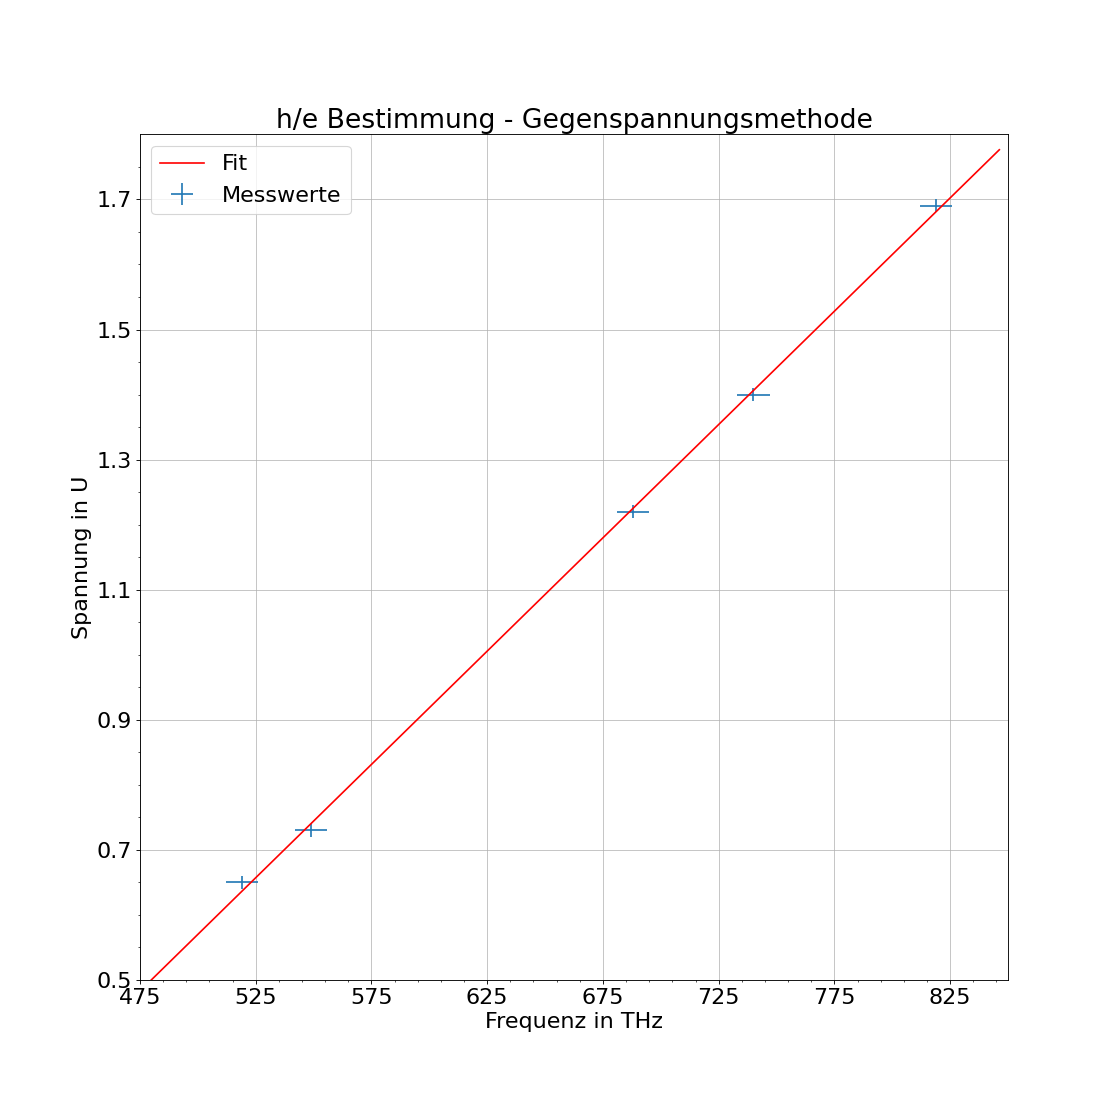
\includegraphics[width=0.8\textwidth]{he_gegenspannung.png}
				\caption{h/e Bestimmung Gegenspannungsmethode}
			\end{figure}
			Aus der Geradenanpassung ging eine Geradensteigung von 
			\begin{equation}
				\frac{h}{e} = (3,48\pm 0,11)\cdot 10^{-15}V s
			\end{equation}
			und ein Ordinatenabschnitt von
			\begin{equation}
				\frac{W_A(A)}{e} = -(1.17\pm 0,07)V
			\end{equation}
			hervor.
		\subsubsection{Direkte Messung}
			Über die direkte Messung ergaben sich folgende Messwerte 
			\begin{figure}[H]
				\centering
				\begin{tabular}{|c|c|c|c|c|c|c|}
					\hline
					Filter & $\lambda$ [nm] & $\Delta\lambda$ [nm] & $\nu$ [THz] & $\Delta\nu$ [THz] & $U_0$ [V] & $\Delta U_0$ [V] \\
					\hline
					1 & 366 & 7 & 819 & 7,8 & 1,68 & 0,01\\
					2 & 405 & 7 & 740 & 6,4 & 1,39 & 0,01\\ 
					3 & 436 & 7 & 688 & 5,5 & 1,18 & 0,01\\
					4 & 546 & 7 & 549 & 3,5 & 0,71 & 0,01\\
					5 & 578 & 7 & 519 & 3,1 & 0,65 & 0,01\\
					\hline
				\end{tabular}
			\end{figure}
			\begin{figure}[H]
				\centering
				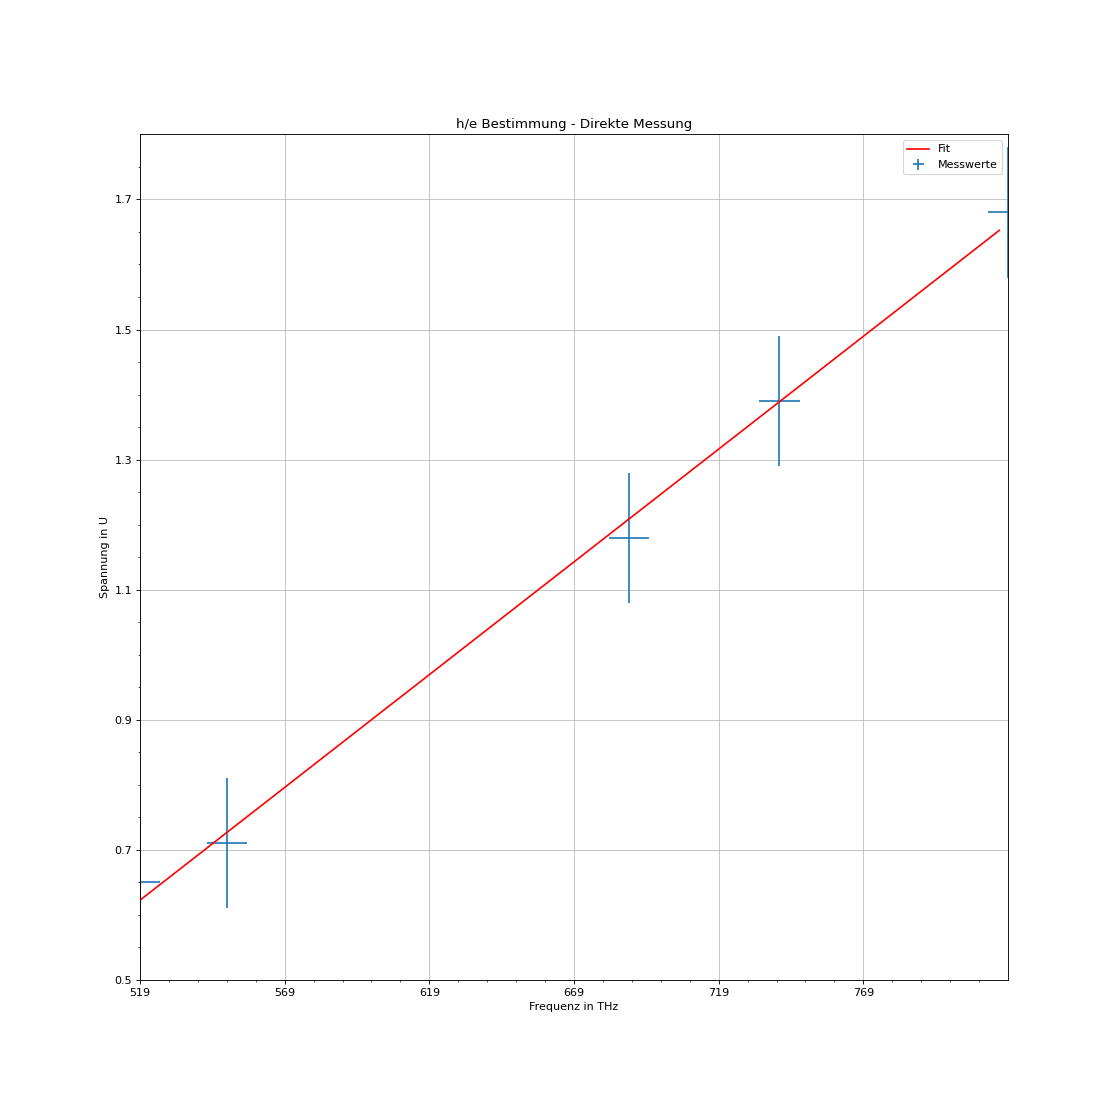
\includegraphics[width=0.8\textwidth]{he_direkt.png}
				\caption{h/e Bestimmung Direkte Messung}
			\end{figure}
			Aus der Geradenanpassung ging eine Geradensteigung von 
			\begin{equation}
				\frac{h}{e}= (3,5\pm 0,1)\cdot 10^{-15}V s
			\end{equation}
			und ein Ordinatenabschnitt von
			\begin{equation}
				\frac{W_A(A)}{e} = (1,17\pm 0,07)V
			\end{equation}
			hervor.
		\subsubsection{Vergleich}
			Beide Methoden liefern uns sehr ähnliche Ergebnisse,
			\begin{figure}[H]
				\centering
				\begin{tabular}{|c|c|c|}
					\hline
					Methode & h/e & $W_A(A)/e$ \\
					\hline
					Gegenspannung & $3,48\pm 0,11$ & $1,17\pm 0,07$ \\
					Direkt & $3,5\pm 0,1$ & $1,17\pm 0,07$ \\
					Literatur & $4,14$ & - \\
					\hline
				\end{tabular}
			\end{figure}

			Jedoch liefert keine der beiden Methoden ein Ergebnis in welchem der Literaturwert liegt. Dennoch lässt sich 
			zur Genauigkeit beider Methoden eine Aussage treffen, da bei der direkten Messmethode nur sehr geringe Ströme fließen
			($R=10^{13}\Omega$ und $V=0-2$ $\Rightarrow I=10^{-13}A$) ist die Messung dieser über ein Messgerät bereits eine Herausforderung
			und kann zu einem starken Problem führen, sobald durch leichte Erschütterungen oder Störfelder diese minimalen Ströme beeinflusst werden.
			Da jedoch in dieser Durchführung beide Methoden vergleichbar genaue Ergebnisse liefern lässt sich die Abweichung vom 
			Literaturwert auf einen konzeptionellen Fehler zurückzuführen wie zum Beispiel die Vernachlässigung der Kathoden-Kontaktspannung.

	\subsection{Intensität und Photostrom}
		In diesem Versuchsteil soll der Zusammenhang zwischen Intensität und Photostrom näher untersucht werden, dafür 
		werden bei bekannter Wellenlänge durch Anwendung verschiedener Graufilter mit verschiedenen Transmissionsgraden
		die Intensitäten Variiert.\\
		Dafür wird die Schaltung der direkten Messung um einen Messverstärker erweitert, welcher den Widerstand
		auf ca. $10^4 \Omega$ reduziert, wodurch Ströme im mA Bereich messbar sind.\\
		Die Messung ergab folgende Werte:
		
		%\begin{table}[H]
		%	\begin{minipage}{.5\textwidth}
		\begin{figure}[H]
			\begin{center}
				\begin{tabular}{|c|c|c|c|c|}
					\hline
						\multicolumn{5}{|c|}{$\lambda$ = 436nm} \\
					\hline
					Filter & T [\%] & $\Delta T$ [\%] & I [$10^{-9}mA$] & $\Delta I$ [$10^{-9}mA$]\\
					\hline
					1 & 68 & 1 & 9,6 & 0,1\\
					2 & 48 & 1 & 6,4 & 0,1\\
					3 & 33 & 1 & 4,9 & 0,1\\
					4 & 28 & 1 & 4,1 & 0,1\\
					5 & 20 & 1 & 2,7 & 0,1\\
					6 & 14 & 1 & 2,1 & 0,1\\
					\hline
				\end{tabular}
			\end{center}
		\end{figure}
			%\end{minipage} 
			%\begin{minipage}{.5\textwidth}
		\begin{figure}[H]
			\begin{center}
				\begin{tabular}{|c|c|c|c|c|}
					\hline
						\multicolumn{5}{|c|}{$\lambda$ = 546nm} \\
					\hline
					Filter & T [\%] & $\Delta T$ [\%] & I [$10^{-9}mA$] & $\Delta I$ [$10^{-9}mA$]\\
					\hline
					1 & 67 & 1 & 3,2 & 0,1\\
					2 & 46 & 1 & 2,2 & 0,1\\
					3 & 31 & 1 & 1,5 & 0,1\\
					4 & 23 & 1 & 1,1 & 0,1\\
					5 & 16 & 1 & 0,8 & 0,1\\
					6 & 11 & 1 & 0,5 & 0,1\\
					\hline
				\end{tabular}
			\end{center}
		\end{figure}

			%\end{minipage}
		%\end{table}
		\begin{figure}[H]
			\centering
			\includegraphics[width=0.8\textwidth]{intensität.png}
			\caption{Intensität und Photonenstrom}
		\end{figure}

		Bei beiden Messungen ist deutlich der lineare Zusammenhang zwischen Transmissionsgrad und Photostrom zu erkennen.
		Auch fällt auf, das Licht mit kleinerer Wellenlänge höhere Photoströme erzeugt, da Photonen dieses Lichts im Allgemeinen
		eine höhere Energie Besitzen. \\
		Eine weitere interessante Beobachtung ist das eintreten des Photoeffekts selbst bei den Niedrigsten Intensitäten, woraus folgt
		, dass das Eintreten des Photoeffekts unabhängig von der Intensität ist. Jedoch steigt die Anzahl der Ereignisse mit der Intensität,
		was auf die Teilchennatur und die höhere Teilchenzahl bei höherer Intensität zurückzuführen ist.\\
		Vergleicht man die Stoppspannung des Aufbaus für 2 verschiedene Transmissionsgrade erhält man folgende Messwerte:
		\begin{figure}[H]
			\centering
			\begin{tabular}{|c|c|c|}
				\hline
				Filter & Transmissionsgrad [\%] & Stoppspannung [V] \\
				\hline
				0 & 100 & $0,72\pm 0,01$ \\ 
				1 & $67\pm 1$ & $0,72\pm 0,01$ \\
				\hline
			\end{tabular}
		\end{figure}
		Man kann direkt aus der Tabelle entnehmen, das die Energie der Transmittierten Photonen nicht beeinträchtigt wird, lediglich die 
		Anzahl wird reduziert. Die kinetische Energie eines Elektrons hängt also nur von der Wellenlänge des Lichts ab, nicht jedoch von
		dessen Intensität. Diese Erkenntnis widerspricht der ursprünglichen Annahme, dass die Intensität 
		des Lichts proportional zur Energie ist.
		

	\subsection{Untersuchung von LEDs mit der Photozelle}
		Eine Praktische Anwendung der oben untersuchten Physikalischen Phänomene ist beispielsweise
		die Bestimmung von Wellenlängen unbekannter Lichtquellen. Hierfür haben wir für 3 LEDs die 
		Stopspannung bestimmt. Diese gibt bei den LEDs jedoch nur die obere Grenze des ca. 30 nm breiten Spektrums an,
		da erst dann eine vollständig Stromfreie Messung zustande kommt.\\
		Die Messung der drei Dioden ergab Folgende Spannungen:
		\begin{figure}[H]
			\centering
			\begin{tabular}{|c|c|c|}
				\hline
				LED & $U_0$ [V] & $\Delta U_0$ [V] \\
				\hline
				1 & 0,99 & 0,01\\
				2 & 0,86 & 0,01\\
				3 & 0,80 & 0,01\\
				\hline
			\end{tabular}
		\end{figure}
		Mit den aus dem ersten Abschnitt gewonnenen Daten lässt sich nun über
		\begin{equation}
			U_0 = \frac{h}{e}\cdot\frac{c}{\lambda} - \frac{W_A(A)}{e} 
			\Leftrightarrow 
			\frac{1}{\lambda} = \frac{eU_0 - e\frac{W_A(A)}{e}}{hc}
		\end{equation}
		\begin{equation}
			\lambda = \frac{hc}{eU_0 - e\frac{W_A(A)}{e}}
		\end{equation}
		mit 
		$$ \frac{h}{e} = (123 \pm 123)$$
		$$ \frac{W_A(A)}{e} = (123 \pm 123)$$
		folgt:
		\begin{figure}[H]
			\centering
			\begin{tabular}{|c|c|c|c|}
				\hline
				LED & $\lambda_{max}$ [nm] & $\Delta\lambda_{max}$ [nm] & Literaturwert \\
				\hline
				1 & 575 & 21 & 570-580 (Gelblich)\\
				2 & 612 & 23 & 595-620 (Orange)\\
				3 & 630 & 24 & 620-780 (Rot)\\
				\hline
			\end{tabular}
		\end{figure}
		Literaturwerte für die Farben wurden von dieser Tabelle\footnote{https://www.hug-technik.com/inhalt/ta/farben entnommen}.
		Allen LEDs konnte eine Farbe zugewiesen werden die im Fehlerbereich liegen. Die bestimmten Wellenlängen sind mit einer 
		Aufspaltung von etwa 20nm im üblichen Bereich für LED Licht. 

\section{Diskussion}
	\subsection{Zu Bestimmung von h/e}
	Der Literaturwert stimmt nicht mit unseren ermittelten Werten überein. Begründet könnte diese 		    Diskrepanz mit der empfindlichen Messapparatur, welche schon durch kleine Stöße ausschlaggebende
	Veränderungen zeigt. 
	
	\subsection{Zu Intensität und Photostrom}
	Anhand der oben abgebildeten Diagramme erkennt man sehr gut die Proportionalität zwischen       		Photostrom und Intensität des Lichts. Auch ist, wie zu erwarten, die Stoppspanung der beiden 		    Messungen gleich. Somit konnten wir in diesem Versuchsteil nachweisen, dass die maximale    kinetische Energie der rausgelösten Elektronen unabhängig von der Intensität des einfallenden Lichts  ist.
	
	\subsection{Zu Untersuchung von LEDs mit der Photozelle}
	Die bestimmten Wellenlängen der verwendeten LEDs stimmen gut mit den Literaturwerten überein. Damit konnte jeder LED eine Farbe zugewiesen werden.




%\begin{thebibliography}{}
%\bibitem[1]{lit1} Versuchsanleitung
%\bibitem[2]{lit2} Quellen
%\bibitem[3]{lit3} Usw
%\end{thebibliography}


\end{document}

%notes:
% Tipler seite 1325 ff
